%&../.preamble
\endofdump

\usetikzlibrary{external}
\tikzset{external/system call={pdflatex --shell-escape --fmt=../.preamble --halt-on-error -jobname "\image" "\endofdump\texsource"}}
\tikzexternalize[prefix=tikz/]

\title{Reti}
\author{Marini Mattia}
\date{$ 1^o $ semestre $ 2^o $ anno}

\begin{document}
\maketitle
\tableofcontents
\newpage

\section{Introduzione ad Internet}
\subsubsection*{Terminologia}
\begin{itemize}
	\item \underline{Host / sistemi terminali / end systems} sistemi (coputer/server) interconnessi
	\item \underline{Clien}: host che invia richieste ad un server, attendendo risposta
	\item \underline{Server}: host che fornisce un determinato servizio da un terminale. I server si trovano nella periferia della rete
	\item \underline{Modem}: dispositivo che converte i bytes in tensioni di corrente che viaggiano sui cavi
	\item \underline{Router}: dispositivo che si occupa di decidere dove i pacchetti vengono spediti. Poco importante per i router domestici, di più per i router che si trovano al centro della rete
	\item \underline{Protocollo}: standard che definisce il formato e l'ordine secondo il quale vengono scambiati messaggi tra due o più entità di comunicazione, così come le azioni intraprese quando i dati vengono inviati/ricevuti. \textit{TCP, IP, HTTP, Skype, Ethernet} sono tutti protocolli
	\item \underline{Internet}: rete delle reti, ossia una rete che connette le diverse reti private
	\item \underline{Servizio affidabile}: servizio che deve garantire che i dati arrivino tutti da sorgente a destinazione, ad esempio quando richiediamo una pagina web
	\item \underline{Servizio best effort}: servizio che non garantisce necessariamente che i dati arrivino tutti da sorgente a destinazione, ad esempio un servizio di \textit{streaming}
	\item \underline{Organismi che gestiscono standard internet}:
	      \begin{itemize}
		      \item \underline{RFC}: REquest for comments
		      \item \underline{IETF}: Internet Engineering Task Force
	      \end{itemize}
	      queste organizzazioni fanno si che due schede di rete di produttori diversi possano comunicare senza problemi
	\item \underline{Architettura peer to peer}: un end system si collega ad un altro end system senza passare per un server
	\item \underline{Architettura client/server}: il client riceve un serviizo da un server. Google, ad esempio, disloca i server in diversi \textit{data center}, nella periferia della rete
	\item \underline{Modem dial-up}
	      \begin{itemize}
		      \item Lento (8/56 kbit/s)
		      \item Non è possibile navigare e telefonare contemporaneamente
	      \end{itemize}
	\item \underline{DSL}
	      \begin{itemize}
		      \item Spesso è \textit{asimmetrica(ADSL)}, ossia vi sono diverse velocità in download e upload
		      \item Fino a 1/5 mbit/s in upstream(upload)
		      \item Fino a 10/20 mbit/s in downstream(download)
	      \end{itemize}
	\item \underline{LAN}, Local Area Network è la rete che collega tutti i dispositivi all'interno di aziende/università. Tutti i dispositivi sono collegati all'edge router
	      \vskip3mm
	      \begin{minipage}[c]{0.48\textwidth}
		      \begin{center}
			      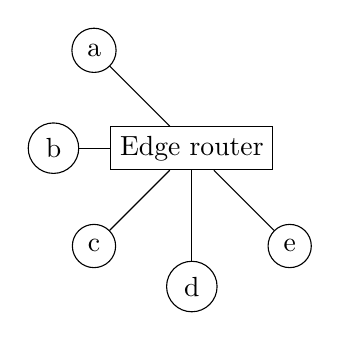
\begin{tikzpicture}[node distance = 5em]
				      \node (r)[draw] at (0,0) {Edge router};
				      \node (a)[circle,draw, above left of = r]  {a};
				      \node (b)[circle,draw, left of = r]  {b};
				      \node (c)[circle, draw, below left of = r]  {c};
				      \node (d)[circle,draw, below of = r]  {d};
				      \node (e)[circle,draw, below right of = r]  {e};
				      \draw (a)--(r);
				      \draw (b)--(r);
				      \draw (c)--(r);
				      \draw (d)--(r);
				      \draw (e)--(r);
			      \end{tikzpicture}
		      \end{center}
	      \end{minipage}
	      %
	      \begin{minipage}[c]{0.48\textwidth}
		      \begin{center}
			      \begin{tikzpicture}[node distance = 3em]
				      \node (r)[draw] at (0,0) {Edge router};

				      \node (inc1)[below of = r, whitedot]  {};
				      \node (inc2)[above left of = r, whitedot]  {};

				      \node (a)[circle,draw, above left of = inc2]  {a};
				      \node (b)[circle,draw, left of = inc2]  {b};

				      \node (c)[circle, draw, below left of = inc1]  {c};
				      \node (d)[circle,draw, below of = inc1]  {d};
				      \node (e)[circle,draw, below right of = inc1]  {e};


				      \draw (a)-|(inc2)-|(r);
				      \draw (b)--(inc2);

				      \draw (c)|-(inc1)--(r);
				      \draw (d)--(inc1);
				      \draw (e)|-(inc1);

				      \node (fit1)[fit = (a)(b)(inc2), dashed, draw]  {};
				      \node (fit2)[fit = (c)(d)(e)(inc1), dashed, draw]  {};
				      \node (coll)[right of = r, anchor = west]  {Collisione per risorse};

				      \draw (coll)|-(fit1.east);
				      \draw (coll)|-(fit2.east);
			      \end{tikzpicture}

		      \end{center}
	      \end{minipage}
	      \vskip3mm
	\item \underline{Reti wireless} possono essere principalmente di due tipi:
	      \begin{itemize}
		      \item \underline{LAN wireless}: il WiFi. In particolare la versioni sono 802.11 a/b/g/n/ac, con corrispettive velocità di 11, 54, 100+ Mbit/s
		      \item Rete di accesso wireless geografica, ad esempio GPS, rete 4g/5g
		      \item Velocità da qualche Mbit fino a 1 Gbit al secondo
	      \end{itemize}
\end{itemize}
\subsection{Struttura reti}
\subsubsection*{Struttura reti domestiche}
\vskip3mm
\begin{tikzpicture}[node distance = 5em]
	\node (m)[draw] at (0,0) {Modem via cavo};
	\node (r)[draw, regular polygon, regular polygon sides = 6, inner sep = 0pt, right of = m, anchor = west]  {Router};
	\node (pc1)[draw, circle, above right of = r] {Pc1};
	\node (pc2)[draw, circle, below right of = r]  {Pc2};
	\node (ap)[draw,chamfered rectangle, right of = r, align = center, anchor = west]  {Punto di accesso\\senza fili};
	\draw (r)|-(pc1);
	\draw (r)|-(pc2);
	\draw (r)--(ap);
	\draw (r)--(m);
	\draw (m.west)--++(-1,0) node ()[anchor = east,align = right]  {da terminazione\\ via cavo};
	\node (fit)[fit = (r)(m), draw, dashed]  {};
	\draw (fit.south) node[anchor = north, align = center]  {spesso stesso\\dispositivo};
\end{tikzpicture}
\vskip3mm
\subsubsection*{Mezzi trasmissivi}
I mezzi sui quali veengono trasmessi i bit possono essere
\begin{itemize}
	\item Mezzi guidati:
	      \begin{itemize}
		      \item RAme
		      \item Fibra ottica
		      \item Cavo coassiale
	      \end{itemize}
	\item Mezzi a onda libera
	      \begin{itemize}
		      \item I segnali si propagano nell'atmosfera o nello spazio, (es wifi, gps)
	      \end{itemize}
\end{itemize}
\subsubsection*{Il cavo}
Tendenzialmente si usa la tecnologia a \underline{doppino intrecciato} o \underline{TP}. Questo è utilizzato per i cavi eternet
\begin{center}
	\tcbox[colback=white]{\includegraphics[width = 0.95\textwidth]{Images/Doppino intrecciato.png }}
\end{center}
I cavi vengono deniminati come segue
\begin{center}
	X / Y TP
\end{center}
\begin{itemize}
	\item \underline{X} è la schermatura dell'intero cavo
	      \begin{itemize}
		      \item  U : unshielded
		      \item  F : foiled (di solito, una lamina di alluminio)
		      \item  S : maglia metallica intrecciata (di solito, rame placcato alluminio)
		      \item  SF : entrambe
	      \end{itemize}
	\item \underline{Y} è la schermatura di ogni doppino
	      \begin{itemize}
		      \item U: unshielded
		      \item F : shielded
	      \end{itemize}
	      Esempi: U/UTP \quad F/UTP \quad S/FTP?
\end{itemize}
\subsection{Il nucleo della rete (core)}
Per trasferire dati da un end system ad un altro end system vi sono principalmente due metodi:
la \underline{commutazione di circuito e la commutazione di pacchetto}
\subsubsection*{Commutazione di circuito}
In questo metodo, le risorse fisiche vengono riservate ai due end systems fino a quando non è finita la transizione di dati. Di fatto il circuito fisico che trasmette i bit viene riservato fino che la comunicazione non termina
\begin{itemize}
	\item Risrse del circuito sono garantite
	\item Risorse non condivise con nessuno
	\item Necssario invio di segnali hand-shake per impostare la connssione (pensa a quando si fa una telefonata)
\end{itemize}
Nello scenario in cui una tratta debba essere divida da più utilizzatori, bisogna capire come spartire le risorse. Vi sono 3 approcci:
\begin{itemize}
	\item \underline{Ripartizione bitrate}: viene suddivisa la banda dedicata a ciascuna connessione (ho 10 Mbit/s, ne do 5 a testa)
	\item \underline{Divisione di frequenza (FDM)}:  ogni utente può utilizzare una data frequenza per quanto tempo gli pare. Ad esempio un canale radio, possiede una frequenza per quanto vuole
	\item \underline{Divisione di tempo (TDM)}: ogni utente può utilizzare tutte le frequenze disponibili per un tempo limitato e definito a priori
\end{itemize}
\begin{esercizio}{Calcolo tempo con TDM}
	Quanto tempo occore per trasmettere $ 640.000 $ bit dall'host $ A $ all'host $ B $ su una rete a \underline{commutazione di circuito}?
	\begin{itemize}
		\item Tutti i collegamenti presentano bit-rate di $ 1536 $ kbit/s
		\item Ciascun collegament utilizza \underline{TDM} con 24 slot/secondo
		\item Si impiegano 500 ms per stabilire la connessione
	\end{itemize}
\end{esercizio}
Risposta:
\begin{itemize}
	\item 24 slot/secondo quindi ogni utente utilizza 1/24 della potenza della rete. Ogni utente ha banda
	      \[
		      \frac{1536}{24} = 64 \frac{kb}{s}
	      \]
	\item Per inviare i dati ho bisogno di
	      \[
		      \frac{640000}{64} = 10 s
	      \]
	\item Per stabilire la connesione servono 500 ms quindi il tempo totale è
	      \[
		      \text{ Tempo totale } = \text{ Tempo connessione } + \text{ Tempo spedizione } = 0.5 + 10 = 10.5 s
	      \]
\end{itemize}
\subsubsection*{Commutazione di pacchetto}
Le risorse possono prendere strade diverse. Per via di congestioni si potrebbe dover aspettare che sia disponibile una linea.
\begin{itemize}
	\item Il traffico di dati viene suddiviso in pacchetti
	\item Ciascun pacchetto utilizza interamente il canale
	\item Le risorse vengono usare a seconda della necessità (\textit{on demand})
\end{itemize}
Questo per certi versi è più efficace che la commutazione di circuito, però possono esserci problemi di \underline{contesa per le risorse}:
\begin{itemize}
	\item La richiesta di risorse può eccdere il quantitativo disponibile
	\item Può esserci una \underline{congestione}. Ciò significa che arriva troppo traffico in arrivo che non riesce ad essere smaltito sufficientemente rapidamente
	\item Ci deve essere \underline{store and forward}. I pacchetti vengono memorizzati mentre attendono di essere spediti
	\item Ogni pacchetto deve essere \underline{ricevuto completamente} prima di essere rispedito per le seguenti ragioni:
	      \begin{itemize}
		      \item Per fare correzione di errori
		      \item Per capire dove va instradato il \footnote{In realtà, nei router moderni possono decidere dove instradare il pacchetto ancora prima che sia completamente ricevuto}{pacchetto}
	      \end{itemize}
\end{itemize}

\begin{tcolorbox}
	La commutazione di pacchetto è l'opzione più utilizzata in quanto:
	\begin{itemize}
		\item E' ottima per spedire dati a raffica in maniera veloce, in quanto ogni host ha a disposizione tute le risorse
		\item Permette di emulare un comportamento \textit{circuit like}, fornendo garanzie sulla larghezza di banda. Tuttavia questo problema è molto complesso e non ancora risolto
	\end{itemize}
	Tuttavia bisogna è necessario dire che:
	\begin{itemize}
		\item La commutazione di pacchetto potrebbe dare problemi di congestione, comportando ritardi e perdite di pacchetti
	\end{itemize}
\end{tcolorbox}

\section{Struttura internet}
Internet possiede una struttura gerarchica:
\begin{itemize}
	\item ISP di livello 1
	      \begin{itemize}
		      \item ISP di livello 2
		            \begin{itemize}
			            \item ISP di livello 3 (\textit{last hop network})
		            \end{itemize}
	      \end{itemize}
\end{itemize}
\begin{center}
	\tcbox[colback=white]{\includegraphics[width=0.95\textwidth]{Images/ISP.png }}
\end{center}
\begin{itemize}
	\item IXP: internet exchange point. Struttura di una terza azienda nella quale gli ISP di livello 2 comprano spazio per router per effettuare peering con altri ISP di livello 2.
	\item ISP di livello 2: grandi compagnie di internet (Vodafone, Telecom...)
	\item PoP: point of presence: Struttura all'interno della quale gli ISP di livello 2 mettono le proprie strutture
\end{itemize}
\subsection{Ritardo trasmissione commutazione di pacchetto}
\begin{center}
	\tcbox[colback=white]{\includegraphics[width = 0.75\textwidth]{Images/Ritardi_commutazione.png }}
\end{center}
\begin{itemize}
	\item Ritardo di elaborazione del pacchetto
	      \begin{itemize}
		      \item Router effetta controllo correttezza dei bit
		      \item Router decide dove inviare i pacchetti
	      \end{itemize}
	\item Ritardo di accodamento
	      \begin{itemize}
		      \item Ritardo che subiscono i pacchetti mentre attendono in coda di essere spediti
	      \end{itemize}
	\item Ritardo di trasmisssione
	      \begin{itemize}
		      \item $ R = $ frequenza di trasmissione in bit/s
		      \item $ L =  $ lunghezza del pacchetto in bit
		      \item Ritardo di trasmissione = $ \frac{L}{R} $
	      \end{itemize}
	\item Ritardo di propagazione
	      \begin{itemize}
		      \item $ d = \text{ lunghezza del collegamento fisico }$
		      \item $ s = \text{ velocità di propagazione del collegamento } $ (m/s)
		      \item $ \text{ Ritardo di propagazione } = \frac{d}{s}$
	      \end{itemize}
\end{itemize}
Quindi possiamo dire che:
\[
	d_{\text {node }}=d_{\text {proc }}+d_{\text {queue }}+d_{\text {trans }}+d_{\text {prop }}
\]

\begin{itemize}
	\item $ d_{\text {proc }}=$ ritardo di elaborazione (processing delay)
	      \begin{itemize}
		      \item 	       in genere pochi microsecondi, o anche meno
	      \end{itemize}
	\item $d_{\text{queue }}=$ ritardo di accodamento (queving delay)
	      \begin{itemize}
		      \item  dipende dalla congestione
	      \end{itemize}
	\item $d_{\text {trans }}=$ ritardo di trasmissione (transmission delay)
	      \begin{itemize}
		      \item  L/R, significativo sui collegamenti a bassa velocità
	      \end{itemize}
	\item $\mathrm{d}_{\text {prop }}=$ ritardo di propagazione (propagation delay)
	      \begin{itemize}
		      \item  da pochi microsecondi a centinaia di millisecondi
	      \end{itemize}
\end{itemize}
Un'altro fattore importante è il ritardo di accodamento. dati
\begin{itemize}
	\item R = frequenza di trasmissione (bit/s)
	\item L = lunghezza del pacchetto (bit)
	\item A = tasso medio di arrivo dei pacchetti (pacchetti/sec)
	      ho che:
\end{itemize}
\[
	\text{ Intensità di traffico } = \frac{L \cdot A}{R}
\]
ossia il rapporto fra la "velocità" con cui entrano dati e la velocità con cui escono
\subsubsection*{Perdita di pacchetti e throughput}
\begin{itemize}
	\item \underline{Perdita di pacchetto}. Nel momento in cui viene inviato un pacchetto ad un rounter il cui buffer è pieno, questo pacchetto viene scartato e dunque perso
	\item \underline{Throughput}. Con throughput si intende "banda", ossia la quantità di bit che possono passare per un determinato collegamento per unità di tempo. Chiaramente vale il principio del collo di bottiglia
\end{itemize}
\subsection{Stratificazione internet}
Internet è strutturato in maniera stratificata. Partendo dall'alto livello per arrivare fino al basso abbiamo i seguenti livelli, ciascuno dei quali fornisce determinati servizi:
\vskip3mm
\hrule
\vskip3mm
\begin{minipage}[c]{0.25\textwidth}
	\begin{center}
		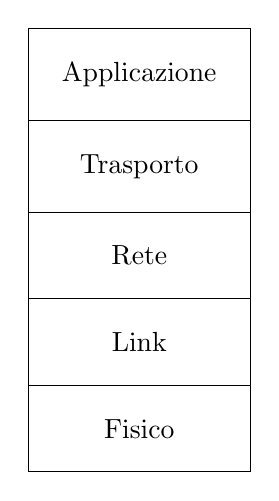
\begin{tikzpicture}
			\node (a)[inner sep = 12pt, anchor = north]at (0,0)  {Applicazione};
			\node (b)[inner sep = 12pt, anchor = north]at (a.south)  {Trasporto};
			\node (c)[inner sep = 12pt, anchor = north]at (b.south)  {Rete};
			\node (d)[inner sep = 12pt, anchor = north]at (c.south)  {Link};
			\node (e)[inner sep = 12pt, anchor = north]at (d.south)  {Fisico};

			\draw (a.north west)rectangle(e.south east -| a.north east);
			\draw (a.north west |- a.south west)--(a.south east |- a.south east);
			\draw (a.north west |- b.south west)--(a.south east |- b.south east);
			\draw (a.north west |- c.south west)--(a.south east |- c.south east);
			\draw (a.north west |- d.south west)--(a.south east |- d.south east);
		\end{tikzpicture}
	\end{center}
\end{minipage}
%
\begin{minipage}[c]{0.60\textwidth}
	\begin{itemize}
		\item \underline{Applicazione} fornisce "API" ad ogni applicazione abbia bisogno di rete. Protocolli FTP, SMTP, HTTP...
		\item \underline{Trasporto} trasferimento dei messaggi a livello di applicazione tra il modulo client e server. Protocolli TCP, UDP
		\item \underline{Rete} fornisce servizi che specificano la strada che i bit (\textit{datagrammi}) prendono. Ip, protocolli di instradamento
		\item \underline{Link} instrada datagrammi verso determinati commutatori di pacchetto (che li spediscono lungo i cavi)
		\item \underline{Fisico} trasmissione di bit su cavi
	\end{itemize}
\end{minipage}
\vskip3mm
\hrule
\vskip3mm
\subsubsection*{Perchè la stratificazion?}
\begin{itemize}
	\item Aiuta ad identificare bene i componenti di un sistema complesso e le inter-relazioni
	\item Facilita la manutenzione e l'aggiornamento del sistema
	      \begin{itemize}
		      \item Modifiche ad un livello risultano trasparenti ad altri livelli
	      \end{itemize}
\end{itemize}
\section{Livello 7: Applicazione}
Fornisce alle applicazioni i mezzi per scambiare dati tramite la rete fornendo servizi quali:
\begin{itemize}
	\item World-wide web (HTTP)
	\item Trasmerimento file (FTP)
	\item Email (POP3, IMAP, SMTP)
	\item Domain Name System (DNS)
	\item File sharing peer-to-peer (P2P)
	\item Terminale virtuale remoto (SSH)
\end{itemize}
L'unita di dato (\textit{data unit}) che viene trasferito a questo livello si chiama \underline{messaggio}
\vskip3mm
Per creare un'applicazione di rete dobbiamo scrivere programmi che:
\begin{itemize}
	\item Girino su più sistemi
	\item Cuminichino attraverso la rete
\end{itemize}
ad esempio, il software di un server web interagisce e comunica con un browser
\subsubsection*{Architettura client-server}
Due componenti: \underline{client} e \underline{server}
\begin{itemize}
	\item Sever
	      \begin{itemize}
		      \item Host sempre attivo
		      \item Indirizzo permanente per accedervi
		      \item Problemi scalabilità (se è molto utilizzato devo avere hardware potente)
	      \end{itemize}
	\item Client
	      \begin{itemize}
		      \item Comunica con il server
		      \item Può avere un indirizzo dinamico
		      \item Non parla con altri client in modo diretto, ma con un server
	      \end{itemize}
\end{itemize}

\subsubsection*{Architettura P2P pura}
\begin{itemize}
	\item Non esiste server, un host, detto \textit{peer}, si connette ad un altro peer in modo diretto
	\item I peer non sono necessariamente sempre attivi e possono cambiare indirizzo ip
\end{itemize}
Difficile da gestire gestire. Il server gestisce tutto mentre qui server qualche sistema diverso
\begin{itemize}
	\item Esiste server centralizzato che gestisce "l'inizializzazione della connessione". Marco viene messo in contatto con Mattia, poi viene stabilito collegamento diretto
\end{itemize}
\subsubsection*{Architettura cloud computing}
\begin{itemize}
	\item Permette di elaborare aarchiviare ed elaborare dati su computer distribuiti e virtualizzati in rete
	\item Sicurezza: i serve sono dislocati, quindi il servizio è garantito ed i dati sono sicuri
	\item \textit{Server farm}: server dislocati, per avvicinarsi all'utente
\end{itemize}
\subsection{Comunicazione processi}
La comunicazione può avvenire fra diversi processi sia all'interno di un computer, sia fra host diversi.
\begin{itemize}
	\item All'interno del computer vengono utilizzati \textit{schemi interprocesso}
	\item Nello scambio fra host la comunicazione avviene tramite \underline{messaggi}
\end{itemize}
\subsubsection*{Socket}
La socket è la "porta" dalla quale passano i messaggi. Ci si può interfacciare ad un socket tramite api che determinano
\begin{itemize}
	\item Quale protocollo viene usato per trasportare i messaggi (es tcp)
	\item Determinati parametri, che vedremo più avanti
\end{itemize}
\subsubsection*{Indirizzi}
\begin{itemize}
	\item  Ogni host ha un indirizzo IP \textit{univoco} a 32 bit, quindi viene rappresentato così:
	      \[
		      \text{ Indirizzo IP: }128.119.245.12
	      \]
	      ossia 4 gruppi da 8 bit, separati da un punto. Ogni gruppo, essendo 8 bit può rappresentare un numero da 0 a 255
	\item Per identificare un processo bisogna conoscere il \underline{numero di porta}, dato che su un server possono girare più processi diversi. Questi numeri tendenzialmente sono standardizzati:
	      \[
		      \text{ N. porta server HTTP: }80
	      \]
\end{itemize}
\subsubsection*{Requisiti servizi di trasporto diverse applicazioni}
In base all'applicazione che dobbiamo implementare, possiamo aver bisogno di diversi requisiti sul trasporto di dati
\begin{itemize}
	\item \underline{Tolleranza alla perdita di dati}: posso lasciarmi qualche bit per strada senza compromettere il servizio?
	\item \underline{Throughput}: devo garantire una determinata larghezza di banda per portare il servizio?
	\item \underline{Sensibilità al tempo}: devo garantire una latenza sufficientemente bassa?
\end{itemize}
\begin{center}
	\tcbox[colback=white]{\includegraphics[width = 0.98\textwidth]{Images/Requisiti trasporto.png }}
\end{center}
\subsection{Protocollid i trasporto: TCP, UDP}
\begin{minipage}[t]{0.48\textwidth}
	\subsubsection*{Transport Control Protocol (TCP)}
	\begin{itemize}
		\item \underline{Orientato alla connessione} richiede processo di connessione fra client e server
		\item \underline{Transporto affidabile}
		\item \underline{Controllo di flusso, e della congestione}: il processo di invio viene "strozzato" per evitare di sovraccaricare il server
		\item \underline{Non offre}: garanzie di banda minima, tempistica e sicurezza
	\end{itemize}
\end{minipage}
%
\begin{minipage}[t]{0.48\textwidth}
	\subsubsection*{User Datagram Protocol (UDP)}
	\begin{itemize}
		\item \underline{Trasferimento inaffidabile}
		\item \underline{Non offre}: setup della connessione e affidabilità. Non offre nemmeno tutto ciò che offre TCP
	\end{itemize}
\end{minipage}

\begin{tcolorbox}
	UDP è un'interfaccia più snella con meno overhead, in quanto non deve  implementare controlli sui dati e offrendo meno features è più veloce e più semplice. Spesso utilizzata per servizi di streaming etc etc
\end{tcolorbox}

\begin{tcolorbox}[colback=white]
	\includegraphics[width = 0.98\textwidth]{Images/TCP UDP.png }
\end{tcolorbox}

\subsection{Protocollo HTTP}
\begin{itemize}
	\item Client inizializza connessione usando \underline{TCP}
	      \begin{itemize}
		      \item Indirizzo ip: \textit{ip server}
		      \item Porta: \textit{80}, per standard
	      \end{itemize}
	\item SErver accetta connesione
	\item Scambio \textit{messaggi}
	\item Chiusura connessione TCP
\end{itemize}
HTTP è un protocollo \underline{stateless}, ossia server non memorizza nessuna richiesta del client
\subsubsection*{Come avviene connessione HTTP - connessione NON persistente}:
Supponiamo di volerci connettere a \textit{www.comeschool.edu/someDep/home.html}. Questo sito contiene 10 immagini.

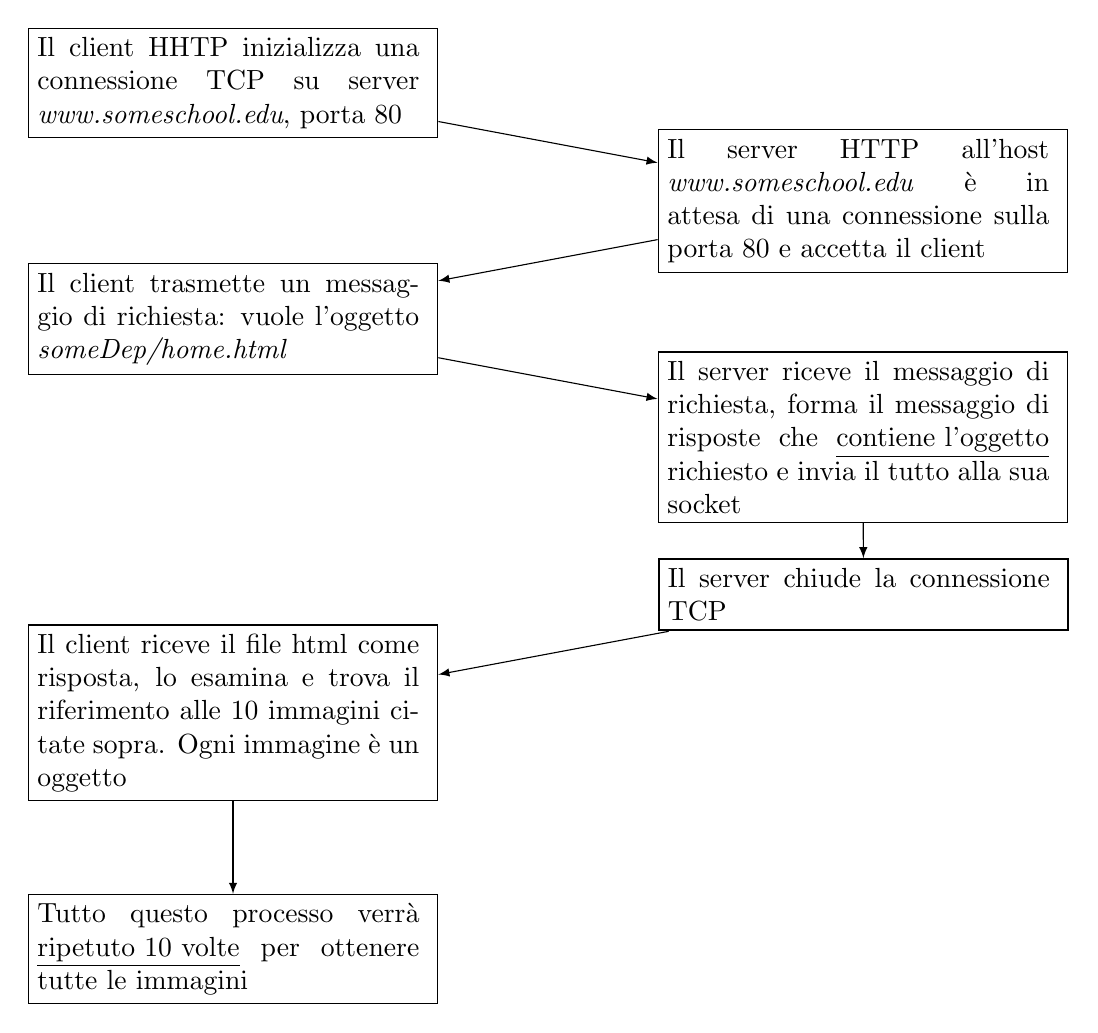
\begin{tikzpicture}
	\node (a)[align = left, anchor = west, draw] at(0,0) {
		\begin{minipage}{0.4\textwidth}
			Il client HHTP inizializza una connessione TCP su server \textit{www.someschool.edu}, porta 80
		\end{minipage}
	};

	\node (b)[align = left, anchor = west, draw] at(8,-1.5) {
		\begin{minipage}{0.4\textwidth}
			Il server HTTP all'host \textit{www.someschool.edu} è in  attesa di una connessione sulla  porta 80 e accetta il client
		\end{minipage}
	};

	\node (c)[align = left, anchor = west, draw] at(0,-3) {
		\begin{minipage}{0.4\textwidth}
			Il client trasmette un  messaggio di richiesta:  vuole l'oggetto \textit{someDep/home.html}
		\end{minipage}
	};

	\node (d)[align = left, anchor = west, draw] at(8,-4.5) {
		\begin{minipage}{0.4\textwidth}
			Il server riceve il messaggio di richiesta, forma il messaggio di risposte che \underline{contiene l'oggetto} richiesto e invia il tutto alla sua socket
		\end{minipage}
	};
	\node (e)[align = left, anchor = west, draw, thick] at(8,-6.5) {
		\begin{minipage}{0.4\textwidth}
			Il server chiude la connessione TCP
		\end{minipage}
	};

	\node (f)[align = left, anchor = west, draw] at(0,-8){
		\begin{minipage}{0.4\textwidth}
			Il client riceve il file html come risposta, lo esamina e trova il riferimento alle 10 immagini citate sopra. Ogni immagine è un oggetto
		\end{minipage}
	};

	\node (g)[align = left, anchor = west, draw] at(0,-11){
		\begin{minipage}{0.4\textwidth}
			Tutto questo processo verrà \underline{ripetuto 10 volte} per ottenere tutte le immagini
		\end{minipage}
	};

	\draw [-latex](a)--(b);
	\draw [-latex](b)--(c);
	\draw [-latex](c)--(d);
	\draw [-latex](d)--(e);
	\draw [-latex](e)--(f);
	\draw [-latex](f)--(g);
\end{tikzpicture}
\vskip3mm
Svantaggio connessioni non persistenti: \underline{per ogni oggetto ho bisogno di 2 round trip time (RTT)}
\begin{itemize}
	\item Overhed sistema operativo
	\item Apertura connessioni TCP in parallelo $ \rightarrow  $ grande utilizzo memoria Crhome
\end{itemize}
Il problema sta nel fatto che la connessione $ TCP $ viene chiusa ogni volta che prendo un oggetto. Qui sta il vantaggio delle connessioni persistenti
prova
\subsubsection*{Messaggi HTTP}
In HTTP vi sono due tipi di messaggi: \underline{richieste e risposte}
\subsubsection*{Messaggio di richiesta}
\begin{itemize}
	\item Messaggi strutturati in maniera testuale (ASCII)
\end{itemize}

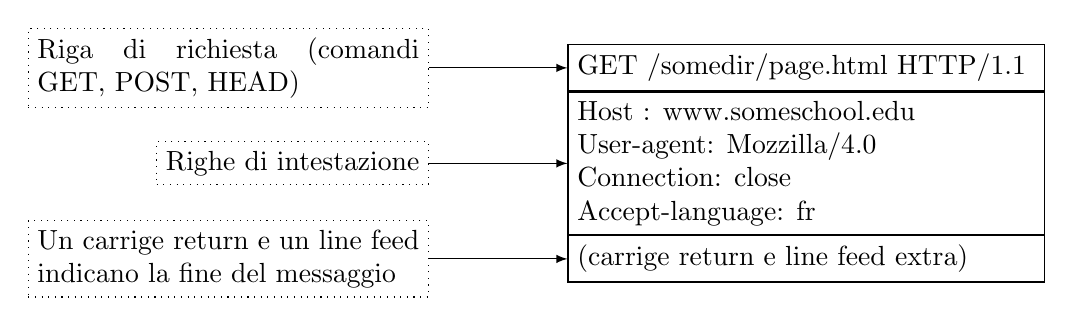
\begin{tikzpicture}

	\node (a)[draw, align = left]at (0,0)  {
		\begin{minipage}{0.47\textwidth}
			GET /somedir/page.html HTTP/1.1
		\end{minipage}
	};
	\node (b)[draw, anchor = north, align = left] at (a.south) {
		\begin{minipage}{0.47\textwidth}
			Host : www.someschool.edu\\
			User-agent: Mozzilla/4.0\\
			Connection: close\\
			Accept-language: fr
		\end{minipage}
	};
	\node (c)[draw, anchor = north, align = left] at (b.south) {
		\begin{minipage}{0.47\textwidth}
			(carrige return e line feed extra)
		\end{minipage}
	};

	\node (1)[xshift = -5em, anchor = east, draw, dotted] at (a.west) {
		\begin{minipage}{0.4\textwidth}
			Riga di richiesta (comandi GET, POST, HEAD)
		\end{minipage}
	};
	\node (2)[xshift = -5em, anchor = east, draw, dotted] at (b.west) {
		Righe di intestazione};
	\node (3)[xshift = -5em, anchor = east, draw, dotted] at (c.west) {
		\begin{minipage}{0.4\textwidth}
			Un carrige return e un line feed indicano la fine del messaggio
		\end{minipage}
	};
	\draw [-latex](1)--(a);
	\draw [-latex](2)--(b);
	\draw [-latex](3)--(c);
\end{tikzpicture}

\begin{center}
	\tcbox[colback=white]{\includegraphics[width = 0.97\textwidth]{Images/Messaggio HTTP.png }}
\end{center}
Comandi:
\begin{itemize}
	\item GET: richiede risorsa dal server tramire URL
	\item POST: invia risorsa al server (es invio dati di un modula o form)
	\item HEAD: richiede risorsa al server, ma non non scarica l'oggetto, ma le informazioni che lo descrivono (dati che descrivono la composizione dell'oggetto, ma non l'oggetto stesso)
	\item PUT: include file nel corpo dell'entità (in giallo) e lo mette all'URL, sempre che vi siano i permessi
	\item DELETE: elimina il fine all'URL, sempre che vi siano i permessi
\end{itemize}
\subsubsection*{Messaggio di risposta}
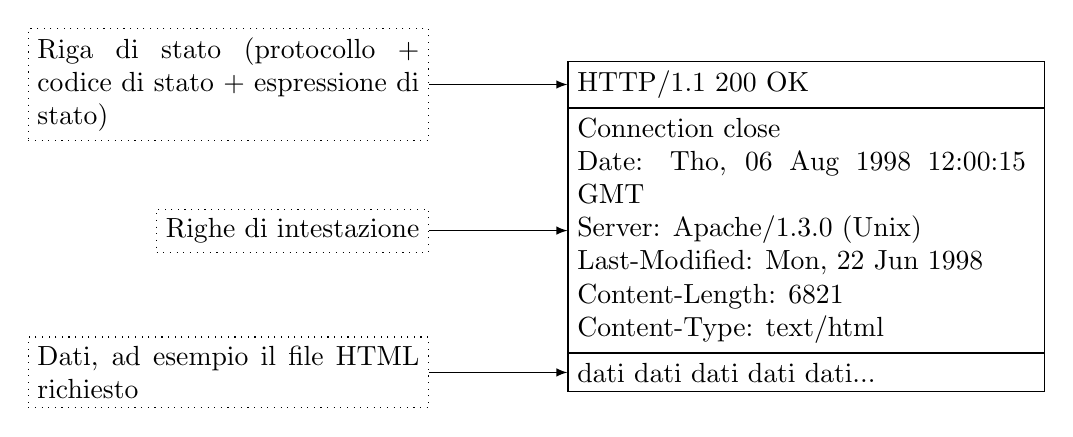
\begin{tikzpicture}

	\node (a)[draw, align = left]at (0,0)  {
		\begin{minipage}{0.47\textwidth}
			HTTP/1.1 200 OK
		\end{minipage}
	};
	\node (b)[draw, anchor = north, align = left] at (a.south) {
		\begin{minipage}{0.47\textwidth}
			Connection close\\
			Date: Tho, 06 Aug 1998 12:00:15 GMT\\
			Server: Apache/1.3.0 (Unix)\\
			Last-Modified: Mon, 22 Jun 1998\\
			Content-Length: 6821\\
			Content-Type: text/html
		\end{minipage}
	};
	\node (c)[draw, anchor = north, align = left] at (b.south) {
		\begin{minipage}{0.47\textwidth}
			dati dati dati dati dati...
		\end{minipage}
	};

	\node (1)[xshift = -5em, anchor = east, draw, dotted] at (a.west) {
		\begin{minipage}{0.4\textwidth}
			Riga di stato (protocollo + codice di stato + espressione di stato)
		\end{minipage}
	};
	\node (2)[xshift = -5em, anchor = east, draw, dotted] at (b.west) {
		Righe di intestazione};
	\node (3)[xshift = -5em, anchor = east, draw, dotted] at (c.west) {
		\begin{minipage}{0.4\textwidth}
			Dati, ad esempio il file HTML richiesto
		\end{minipage}
	};
	\draw [-latex](1)--(a);
	\draw [-latex](2)--(b);
	\draw [-latex](3)--(c);
\end{tikzpicture}
\section{Termini}
\begin{itemize}
	\item Directory server: server di un'architettura P2P a cui ogni peer comunica le risorse che ha da offrire e di cui ha bisogno
	\item Super nodo o ultra peer: nodo in architettura peer to peer che funge da directory server. Determinato dinamicamente da algoritmi
	\item Architettura P2P ibrida: P2P con super nodi
	\item Scalabilità verticale o orizzontale: rispettivamente aggiungere più risorse allo stesso server o piùs erver
	\item Rete single homed-multi homed
	\item IXP: internet exchange point, serve a far comunicare isp di livello 2 direttamente fra di loro
	\item CDN enter deep e bring home: la prima installa server negli ISP, la seconda negli IXP
	\item HTTP: livello applicazione porta 80
	\item Struttura HTTP:
	      \begin{itemize}
		      \item Richiesta : \textit{Metodo - percorso - verione}
		            \begin{itemize}
			            \item Metodo: \textit{GET, POST, PUT, DELETE, HEAD, OPTIONS, TRACE}
		            \end{itemize}
		      \item Risposta \textit{Versione - codice stato - Espressione stato}
		            \begin{itemize}
			            \item Codice di stato = numero
			            \item Espressione di stato = descrizione numero
		            \end{itemize}
	      \end{itemize}
	\item Binary framing: livello intermedio di HTTP 2.0 che modifica la codifica dei messaggi, rendendolo incompatibile con HTTP 1.0 / HTTP1.1
	\item FTP: livello applicazioe porta 21 per comandi e 22 per files
	\item SMTP, POP3, IMAP3. Scambio messaggi fra host online, scarico messaggi senza memoria, riorganizza messaggi creando cartelle con memoria. SMTP ha porta 25
	\item TLS : protocollo che aggiunge autenticazione e sicurezza sul passaggio di  dati da associare a quelli sopra. Numeri di porta differenti da protocolli senza TLS in quanto non posso comunicare poste con TSL con poste senza
	\item STARTLS: TLS ma su porte standard
	\item Server DNS : TLD (top level domain (.com)), SLD (second level domain (google)). \textit{Roor server(13) $ \rightarrow  $ TDL server $ \rightarrow  $ Authoritative server $ \rightarrow  Server ISP $}
	\item Resolver: parte del OS che risolve nomi host
	\item RR: Resource record \textit{(name, value, type, ttl)}
	\item Checksum: sommo parole 16 bit e faccio complemento a 1
	\item Trasmissione sicura:
	      \begin{itemize}
		      \item Stop and wait: mando pacchetto aspetto relativa ack e ripeto
		      \item Go back n: pipeline con massimo n pacchetti insieme. Quando parte un pacchetto parte un timer. I pacchetti vengono ricevuti in ordine e quelli in disordine vengono scartati. Vengono inviati in ordine fino a quando non scatta timeout. In quel casi vengono rinviati da pacchetto perso
		      \item Selective repeat
		            \begin{itemize}
			            \item Mittente: tiene traccia di quali pacchetti sono stati inviati e di quali è stato ricevuto ack. Invia ogni volta il più basso non inviato. Slitta finestra quando ho ricevuto un ack per i primi k elementi di $ W_T $
			            \item Ricevitore: tiene traccia dei pacchetti arrivati. Slitta $ W_R $ ogni volta che sono arrivati i primi $ k $ pacchetti
			            \item Vale che $ \left|W_T\right| + \left|W_R\right| \le n_{seq}$ dove $ n_{seq} $ è massimo numero di pacchetto (pacchetti numerati da $ 0 $ a $ n_{seq} $). Questo perchè nel peggiore dei casi (perdo tutti ack di ritorno), $ W_T $ e $ W_R $ sarebbero messe così: $ \underbracket[0.1ex]{1,2,3, 4}_{W_T}, \underbracket[0.1ex]{5,6,7,8}_{W_R} $, quindi se la somma della loro dimensione fosse maggiore di $ n_{seq} $, allora l'id del pacchetto non sarebbe più univoco e rischierei di accettare pacchetti diversi da quelli effettivamente desiderati
		            \end{itemize}
	      \end{itemize}
	\item TCP:
	      \begin{itemize}
		      \item Init: \textit{SYN}, chiusura: \textit{FIN}, chiusura brusca: \textit{RST}
		      \item Raggruppa in MSS \textit{maximus segment size}, che dipende da MTU \textit{maximum transmit unit} del livello sottostante
		      \item RTO: \textit{retransmission time out}
		            \[
			            \text { EstimatedRTT }=(1-\alpha) \cdot \text { EstimatedRTT }+\alpha \cdot \text { SampleRTT } \text { per } \alpha=0.125
		            \]
		            \[
			            \operatorname{DevRTT}=(1-\beta) \cdot \operatorname{DevRTT}+\beta \cdot \mid \text { SampleRTT }- \text { EstimatedRTT } \mid \text { per } \beta=0.25
		            \]
		            \[
			            R T O=\text { EstimatedRTT }+4 \text { DevRTT }
		            \]
		            Se invece non vi sono misure:
		            \[
			            \text{EstimatedRTT} = \text{ SampleRTT } \quad \text{ DevRTT } = 1/2\text{ SampleRTT } \quad \text{ RTO } = \text{ 1 sec}
		            \]
	      \end{itemize}
	\item AIMD:
	      \begin{itemize}
		      \item Incremento di 1 MSS finche non perdo pacchetti. Quando perdo, dimezzo CWND
		      \item Si ottiene fairness: banda tende a ripartizione equa
		      \item Slow start:
		            \begin{itemize}
			            \item Incrementa ogni ack ricevuto di 1 MSS (esponenzialmente)
			            \item Quando raggiunge SSTHRESH (Slow Start Threshold )passa a congestion avoidance
		            \end{itemize}
		      \item Congestion avoidance
		            \begin{itemize}
			            \item Aumeta CWND di $ \frac{1}{\text{ CWND }} $ segmenti per ogni ack ricevuto
			            \item Se ricevo tutti ack, allora aumento di 1 segmento ogni RTT
		            \end{itemize}
		            i
	      \end{itemize}
	\item Fast retransmit e fast recovery
	      \begin{itemize}
		      \item Al terzo ack duplicato entro in fast recovery.
		            \begin{itemize}
			            \item RESTORE contiene ultimo segmento del quale si è ricevuto ack che dovrebbe essere stato trasmesso prima di entrare in fast recovery
			            \item Per ogni ack duplicato aumento CWND di 1
			            \item Appeka arriva un ack superiore o uguale a RESTORE, riprendo a trasmettere con
			                  \begin{itemize}
				                  \item CWND = CWND/2 + 3
				                  \item SSTRESH = CWND / 2
			                  \end{itemize}
		            \end{itemize}
	      \end{itemize}
	\item Alternative a Fast retransmit:
	      \begin{itemize}
		      \item CUBIC:  simile  a fast retransmit su RTT bassi. invece che dimezzare CWND fa CWND = 0.7 CWND

		      \item BRR: protocollo serer side di google, sfrutta concetto collo di bottiglia
		      \item QUIC: emula TCP + TLS usando UDP, ma evita di effettuare doppio handshake
	      \end{itemize}
\end{itemize}

\subsection{Rete}
\begin{itemize}
	\item Funzione piano dati:  decide come fare \textit{forwarding} localmente, ossia come passare un pacchetto da una porta di ingresso ad una di uscita
	\item Funzioni piano controllo: insieme di algoritmi che determinano percorso da prendere (\textit{routing})
	\item \textit{Terminatore di linea - protocollo data link (ethernet) - buffer di inoltro - sistema di commutazione}
	\item Sistemi di commutazione:
	      \begin{itemize}
		      \item A memeoria: leggo e scrivo su memoria, 2 accessi a sistema
		      \item A bus: uno per volta sul bus condiviso
		      \item A matrice: più pacchetti alla volta
	      \end{itemize}
	\item HOL: \textit{Head of line block}, quando il nodo non calcola abbastanza in fretta
	\item Porta di uscita:
	      \begin{itemize}
		      \item FIFO or \textit{priority} scheduling
		      \item Pacchetti scartati con \textit{tail drop - priority drop - random drop}
	      \end{itemize}
	\item Frammentazione
	      \begin{itemize}
		      \item Flags M \textit{more fragments} e D \textit{do not fragment}
		      \item Non usata per ragioni di sicurezza (Attacchi Ddos o overlapping fragments)
	      \end{itemize}
	\item Registrar: autorita che possono assegnare indirizzi ip e nomi id dominio
	\item Indirizzi ip:
	      \begin{itemize}
		      \item \textit{Subnet mask, default gateaway}
		      \item NAT: apparecchio che associa indirizzo ip privato ad uno pubblico
		            \begin{itemize}
			            \item Rompe encapsulation livelli (modifica porte livello trasporto e ip livello rete)
			            \item Per comunicare a server serve port forwarding
		            \end{itemize}
		      \item Indirizzi:
		            \begin{itemize}
			            \item Privati: 10.0.0.0/8, 172.16.0.0/12, 192.168.0.0/16
			            \item Indirizzi di rete: la parte dopo la subnet mask è tutta zero
			            \item Indirizzo broadcast: la parte dopo la subnet mask è tutta uni
			            \item Broadcast locale: tutti uni (il pacchetto non va fuori dalla rete locale)
			            \item Indirizzo "questo computer": tutti zeri
			            \item Indirizzi loopback: 127.0.0.0/8 per testare app di rete
			            \item Indirizzi multicast: iniziano con 1110, come broadcast
			            \item Link local: 169.254.0.0/16, vengono assegnati in modo random a disposivi ai quali non è possibile assegnare ip
		            \end{itemize}
	      \end{itemize}
	\item ARP
	      \begin{itemize}
		      \item Serve per scoprire un indirizzo MAC (HADDR) associato ad un indirizzo ip (PADDR)
		      \item I messaggi arp vengono trasmessi in broadcast e solo il dispositivo di interesse risponde
		      \item Arp caching: le risponde arp vengono salvate 30 sec e sovrascritte dalle più recenti
	      \end{itemize}
	\item ICMP: \textit{internet control message protocol}
	      \begin{itemize}
		      \item Serve per recuperare informazioni e segnalare errori
		      \item Ping: viene sfruttato il meccanismo id \textit{echo reply}
		      \item Traceroute: vengono mandati pacchetti con TTL incrementali. Ogni volta che il pacchetto scare viene inviata risposta
	      \end{itemize}
	\item DHCP: \textit{dynamic host configuration protocol}
	      \begin{itemize}
		      \item DHCP discover
		      \item DHCP offer
		      \item Client accetta richiesta
		      \item DHCP ack
		      \item Utilizzo indirizzi broadcast 255.255.255.255 perchè client non ha ancora ip
		      \item Transaction id inclusa in messaggio per sapere a chi è riferito broadcast
		      \item Usa UDP (connessione impossibile vista assenza di ip)
		      \item Se non esiste serve DHCP, allora si assegnano indirizzi link-local, e ogni volta si manda messaggio arp. Se nessuno risponde vuol dire che ip non è utilizzato
	      \end{itemize}
\end{itemize}
\subsubsection*{Protocolli di routing}
\begin{itemize}
	\item OSPF: sfrutta \textit{multicast} 224.0.0.5
	      \begin{itemize}
		      \item \textit{Hello - exchange - flooding} verifica router adiacenti - comunica ai ruoter adiacenti stato rete - comunica a tutti i router ricorsivamente stato rete
		      \item Dijkstra
		      \item Gerarchia: rete \textit{dorsale} e \textit{reti di area}
	      \end{itemize}
	\item Dijkstra - \textit{link state}
	\item Bellman ford - \textit{distance vector}
	\item Count to infinity: quando un collegamento viene modificato si viene fatti rimbalzare fra due nodi all'infinito. Soluzioni:
	      \begin{itemize}
		      \item Settare \textit{max hop} (di solito 15)
		      \item Split horizon - X non manda a Y le rotte apprese da Y stesso
		      \item Poison reverse - se X passa da Y per arrivare a Z, allora X informa Y che la sua distanza da Z è $ \infty  $
	      \end{itemize}
	\item RIP: \textit{UDP, porta 520, muticast su 224.0.0.9, processo routed, usa poisoned reverse}, simile a Distance vector. Quando un nodo non riceve aggiornamenti per 180 il link si da per rotto
\end{itemize}
\subsection{BGP}
\begin{itemize}
	\item \textit{BPG speakers} si inviano \textit{path vectors} con destinazione, next hop e path
	\item Connessione client-provider, viceversa o peer to peer
	\item \textit{Ingress policies - egress policies}, filtrano in entrata e uscita. I persorsi accettati sono salvati rispettivamente in tabelle ADJ\_RIB\_IN e ADJ\_RIB\_OUT
	\item Messaggi Open, Notification, KeepAlive e Update.
	      \begin{itemize}
		      \item Open apre connessione. Connessione è effettivamente aperta dopo ever ricevuto keepalive
		      \item Notification: informa BPG speaker di un errore
		      \item Update: \textit{Addittive o sottrattive (withdraw)}: aggiungono o rimuovono rotte
	      \end{itemize}
\end{itemize}
\subsection{Livello data link}
\begin{itemize}
	\item Servizi di \textit{consegna affidabile - controllo flusso - rilevamento e correzione degli errori}
	\item Collegamento \textit{half duplex o full duplex}, rispettivamente uni/bi direzionale
	\item Correzione errori:
	      \begin{itemize}
		      \item Bit di parità unidirezionale: sgama errori, bidirezionale permette di correggerli
		      \item Ridondanza e interleaving: ogni bit viene ridondato e riordinato in maniera casuale. All'arrivo i bit vengono rimessi nell'ordine originale e per ogni gruppo si sceglie il bit ripetuto di più
		      \item
	      \end{itemize}
	\item TDMA, FDMA, CDMA: in quest'ultimo viene assegnato un \textit{chip}, e viene inviato lo xor fra dati e chip. Al destinatario viene ancora fatto xor. Se il dato non corrisponde allo xor giusto si ottiene solo rumore
	\item Slotted ALOHA: ogni trasmettitore è sincronizzato e può trasmettere solo 1 alla volta. Avendo $ N $ trasmettitori il numero massimo di pacchetti è
	      \[
		      N * p\left(p-1\right)^{N-1}
	      \]
	      il valore di $ p $ che massimizza l'espressione sopra è $ \frac{1}{n} $ e il limite per $ N \to  \infty  $ è :
	      \[
		      \lim_{n \to \infty} \left(1 - \frac{1}{N}\right)^{ N-1} = \frac{1}{e} \approx 0.36
	      \]
	      Se ALOHA non fosse slotted, la trasmissione massima sarebbe circa $ \frac{1}{2e} \approx 0.18 $, ossia la metà dello slotted
	\item CSMA p-persistente (\textit{carrier sense multiple acces}): quando canale occupato aspetta fino a quando non è libero e poi con probabilità $ p $ trasmette segnale
	      \begin{itemize}
		      \item Finestra di vulnerabilità: periodo in cui non è certo che nodo sia libero o occupato. Tempo di propagazione + tempo necessario per rilevare collisione
		      \item Efficace quando tempo di propagazione è molto inferiore a tempo trasmissione
		      \item In reti cablate: CSMA/CD quando rilevo collisione invio subito segnale
		      \item In reti wireless: CSMA/CA: si procede a tentoni, riducendo $ p $(probabilità collisione) in base a proprietà rete
	      \end{itemize}
	\item Protocolli a turni:
	      \begin{itemize}
		      \item Polling: \textit{master} invia poll a \textit{slave} e slave risponde con dati. Problema SPOF e inefficiente
		      \item Token: onferisce abilità di trasmettere e viene passato fra host. Stessi problemi polling
		      \item Ethernet:
		            \begin{itemize}
			            \item Inizialmente \textit{bus} e \textit{vampirizzazione} con \textit{terminatori}
			            \item Poi \textit{HUB} con \textit{switch}
			            \item Doppino incrociato con connettore \textit{rj45}
			            \item No connesso no sicuro no ack
			            \item Protocollo MAC CSMA/CD unslotted
			            \item Ogni collisione si sceglie valore di backof fra 0 e $ \left(2^{k}-1\right)T $
			                  con $ k \le 7 $ e $ T =$ tempo per trasmettere 512 bit
		            \end{itemize}
	      \end{itemize}
	\item Domini:
	      \begin{itemize}
		      \item Di collisione: hub $ \rightarrow  $1, switch $ \rightarrow  $ tanti quante le porte
		      \item Di broadcast: mappatura 1:1 con domini di collisione
	      \end{itemize}
	\item Switch:
	      \begin{itemize}
		      \item \textit{backward learning}, aggiorna route corrispondente a mac sorgente
		      \item Se pacchetto ha dest === src viene scartato
		      \item Problema dei loop, finisce in flooding infinito, risolto da STP
	      \end{itemize}
	\item STP: \textit{spanning tree protocol}
	      \begin{itemize}
		      \item Struttura logica è spanning tree $ \rightarrow  $ no cicli. Struttura fisica ha loops (ridondata)
		      \item Ogni switch è identificato da 16 bits (impostati da amministratore rete) + 48 bits MAC address
		      \item Pacchetti di controllo \textit{BPDU}
		      \item Ogni porta può essere: \textit{bloccata, designata, radice}
	      \end{itemize}
	\item LAN: per performance o separazione degli intenti
	      \begin{itemize}
		      \item Impossibile identificare gruppi $ \rightarrow  $ introduzione nuovo protocollo ethernet
		      \item Campo \textit{VLAN identifier} in header
		      \item Se host non supporta vlan no problem: switch manipola headers
		      \item Se switch non supporta vlan problemi: o scarta frame, o inoltra senza considerare vlan
	      \end{itemize}
	\item Reti wireless:
	      \begin{itemize}
		      \item Ad hoc (tipo bluetooth) o a infrastruttura (tipo wifi)
		      \item \textit{(ESS (BSS AP)(BSS AP))}
		            \begin{itemize}
			            \item WLAN: \textit{Wireless Local Area Network}
			            \item Extended service point
			            \item Basic service point
			            \item Acces point
		            \end{itemize}
		      \item Standard wifi
		            \begin{itemize}
			            \item 2.4 ghz divisi in 11 canali
			            \item Associazione passiva o attiva
			            \item Invio \textit{beacon} con SSID, indirizzo MAC
			            \item Assegnazione ip sottorete tramite DHCP
			            \item Attenuazione del segnale viaggia come $ r^2  $
			            \item Non può ricevere e inviare contemporaneamente (autointerferenze)
		            \end{itemize}
	      \end{itemize}
\end{itemize}
\end{document}
